\documentclass[12pt,a4paper]{article}

% -------------------------------------------------
% OSNOVNE NASTAVITVE
% -------------------------------------------------
\usepackage[utf8]{inputenc}
\usepackage[T1]{fontenc}
\usepackage[slovene]{babel}
\usepackage{lmodern}
\usepackage[a4paper,margin=2.5cm]{geometry}
\usepackage{setspace}
\onehalfspacing

\usepackage{amsmath,amssymb}
\usepackage{booktabs}
\usepackage{array}
\usepackage{tabularx}
\usepackage{graphicx}
\usepackage{float}
\usepackage{caption}
\usepackage{url}
\usepackage[hidelinks]{hyperref}
\usepackage{csquotes}

% Grafi neposredno iz CSV
\usepackage{pgfplots}
\pgfplotsset{compat=1.18}

\usepackage{array}
\usepackage{float}

% Literatura
\usepackage[
    backend=biber,
    style=authoryear,
    sorting=nyt
]{biblatex}
\addbibresource{viri.bib}

% -------------------------------------------------
% PODATKI O NALOGI
% -------------------------------------------------
\title{\textbf{Umetna inteligenca kot vir raziskav in razvoja ter dolgoročne gospodarske rasti:}\\
ZDA v obdobju 2010--2025}
\author{
Andraž Ajdovec \and Tin Cvek \and Jan Hrovat \and Miha Ručigaj
}
\date{oktober, 2026}

\begin{document}

\maketitle
\thispagestyle{empty}

\vfill
\begin{center}
Predmet: Makroekonomija\\
Seminarska naloga\\
Univerza: \textit{Fakulteta za matematiko in fiziko}\\
Mentor: \textit{Jan Grobovšek}
\end{center}
\vfill

\newpage
\tableofcontents
\newpage



\section{Uvod}\label{sec:uvod}

\subsection{Širši okvir in pomen problematike}
Teorija rasti je osrednja makroekonomska tema \parencite[str.~1]{polanec_rast}, saj je rast po presoji avtorjev učbenika za blaginjo dolgoročno pomembnejša od nihanj poslovnega cikla \parencite[str.~5]{garin2021}. Že majhne razlike v povprečni stopnji rasti se skozi čas močno seštejejo: ena odstotna točka višja rast v štiridesetih letih pomeni približno 49~\% višjo raven dohodka na prebivalca ($1{,}01^{40}\approx 1{,}49$) \parencite[str.~4]{polanec_rast}.

Solow--Swanov model pokaže, da povečanje stopnje varčevanja ne ustvari trajne rasti in da na dolgi rok rast outputa na delavca določa le rast tehnologije oziroma produktivnosti \parencites[str.~13--14]{polanec_rast}[str.~108]{garin2021}. Ker model to rast privzame kot eksogeno, je ne pojasni \parencites[str.~18]{polanec_rast}[str.~129]{garin2021}. Produktivnost je pomembna tudi za razlike v dohodku med državami, ki jih učbenik pripisuje predvsem razlikam v skupni faktorski produktivnosti (TFP) \parencite[str.~143--144]{garin2021}. TFP pri tem ni neposredno opazljiva, temveč jo merimo kot ostanek, ki ga ne pojasnijo merljivi inputi dela in kapitala (Solowov rezidual) \parencites[str.~22]{polanec_rast}[str.~142]{garin2021}.

Vir produktivnosti je zato treba iskati zunaj Solow--Swanovega modela. To počne teorija endogene rasti, po kateri je tehnološki napredek rezultat namernih vlaganj v znanje in raziskave, ki se povrnejo iz prihodnjih dobičkov \parencite[str.~18]{polanec_rast}. Raziskave in razvoj (R\&R) so po zapiskih lahko pomemben vir rasti TFP: navedene ocene govorijo o do 66~\% rasti TFP \parencite[str.~28]{polanec_rast}. Umetna inteligenca (UI) v nalogi nastopa kot možen dejavnik, ki poveča učinkovitost raziskovalnega procesa in bi tako po mehanizmu endogene rasti lahko zvišala nastajanje znanja in TFP. To je izhodiščna predpostavka, ki jo preizkušamo, ne uveljavljena ugotovitev. Učinek tudi ni nujno takojšen: splošnonamenske tehnologije zahtevajo komplementarne investicije in učenje, zato je rast sprva lahko počasnejša \parencite[str.~28]{polanec_rast}.

\subsection{Predstavitev izbranega primera: ZDA v obdobju 2010--2025}
Za empirični del smo izbrali ZDA. Po podatkih NCSES so skupni izdatki za R\&R leta 2023 znašali približno 937 milijard USD, ocena za 2024 pa je 993 milijard USD \parencite{ncses2026}. Zapiski navajajo, da se več kot 95~\% svetovnih R\&R izvaja v razvitih državah \parencite[str.~31--32]{polanec_rast}. ZDA so med vodilnimi državami, zato je njihova dolgoročna rast v obravnavanih modelih pretežno odvisna od rasti produktivnosti in ne od dohitevanja: država v ustaljenem stanju raste le toliko, kot raste produktivnost \parencite[str.~130,~135]{garin2021}, med razvitimi državami pa bolj razvite rastejo počasneje kot manj razvite \parencite[str.~5--6]{polanec_rast}. Gre za našo interpretacijo teh virov.

Obdobje 2010--2025 razdelimo na tri podobdobja (2010--2014, 2015--2019 in 2020--2025). To je razdelitev za potrebe primerjave in ne zgodovinska periodizacija razvoja UI. Pri razlagi je treba upoštevati, da se je generativna UI množično razširila šele po izidu orodja ChatGPT 30.~novembra 2022 \parencite{openai2022}, da začetek zadnjega podobdobja (2020--2022) zaznamuje pandemija ter da se serije R\&R in UI-patentov končajo prej kot serija TFP (v naši analizi leta 2023). Podatki o R\&R in patentih zato zajemajo generativno UI le za eno leto.

V analizi spremljamo gibanje izdatkov za R\&R, federalna vlaganja v UI, ustvarjanje novega znanja prek UI-patentov ter razvoj TFP.

\subsection{Raziskovalno vprašanje in hipoteze}
\noindent\textbf{Glavno raziskovalno vprašanje:} Katera od hipotez o vlogi umetne inteligence v procesu gospodarske rasti je najbolj skladna z gibanjem izdatkov za R\&R, UI-patentov in TFP v ZDA v obdobju 2010--2025?

Na to vprašanje odgovorimo prek treh podvprašanj:
\begin{enumerate}
    \item Ali so se raziskovalni inputi, merjeni s skupnimi izdatki za R\&R in federalnimi vlaganji v UI, povečali?
    \item Ali je naraščala inovacijska aktivnost, merjena z UI-patenti?
    \item Ali se je rast TFP pospešila in ali je velikost sprememb v skladu s tem, kar bi lahko pričakovali od UI?
\end{enumerate}

Za odgovor v poglavju~\ref{sec:teorija} opredelimo štiri hipoteze: H1 (UI ne spremeni dolgoročne rasti) \parencite[str.~13]{polanec_rast}, H2 (UI poveča stopnjo tehnološkega napredka) \parencites[str.~14--15]{polanec_rast}[str.~108--109]{garin2021}, H3 (UI poveča raziskovalne inpute ali njihovo produktivnost) \parencite[str.~27--28]{polanec_rast} in H4 (UI poveča donose znanja tako, da se rast pospešuje) \parencite[str.~26--27]{polanec_rast}. Ne poskušamo dokazati vzročnosti, temveč preverjamo, katera hipoteza je z opaženimi trendi najbolj skladna in kaj bi jo ovrglo. Pri tem so pomembne tri omejitve: TFP je ostanek, v katerem končajo tudi napake merjenja inputov \parencite[str.~23--24]{polanec_rast}, neposrednih podatkov o zasebnih vlaganjih v UI nimamo, UI-patenti in federalna vlaganja pa pokrivajo le del dejavnosti.

\subsection{Struktura naloge}
V poglavju~\ref{sec:podatki} predstavimo uporabljene podatke in analiziramo razvoj izdatkov za R\&R, federalnih vlaganj v UI, UI-patentne aktivnosti ter TFP v ZDA. V poglavju~\ref{sec:teorija} predstavimo teoretični okvir gospodarske rasti, pri čemer se osredotočimo na Solow--Swanov model, računovodstvo gospodarske rasti, teorijo endogene rasti in hipoteze o vlogi UI. V poglavju~\ref{sec:uporaba} napovedi hipotez primerjamo z opaženimi podatki, v poglavju~\ref{sec:zakljucek} pa podamo kritično presojo ugotovitev, izpostavimo omejitve analize in odgovorimo na raziskovalno vprašanje.

\section{Teoretični okvir gospodarske rasti}\label{sec:teorija}
Poglavje predstavi, kaj teorija pove o virih dolgoročne rasti, kako se TFP meri in kako lahko UI vstopi v modele rasti. Iz tega izpeljemo štiri hipoteze H1--H4, ki jih v poglavju~\ref{sec:uporaba} primerjamo s podatki.

\subsection{Viri dolgoročne rasti}\label{sec:viri}
Dolgoročno rast lahko razlagamo z akumulacijo proizvodnih dejavnikov, predvsem fizičnega in človeškega kapitala, ali z rastjo skupne faktorske produktivnosti (TFP). Ta po zapiskih odraža novo tehnologijo, pa tudi institucije, delež države v BDP in odprtost mednarodni trgovini \parencite[str.~8]{polanec_rast}. Učbenik med dejavniki produktivnosti našteva izobrazbo, institucije, finančni sistem, trgovino in infrastrukturo \parencite[str.~144--145]{garin2021}. Gibanja TFP zato ni mogoče samodejno pripisati eni sami tehnologiji; to omejitev upoštevamo pri preizkusu hipotez. Človeški kapital je znanje, utelešeno v delavcih, tehnologija pa je v zapiskih opisana kot načrt (angl.~\emph{blueprint}), torej zapis, kako se proizvod proizvaja \parencite[str.~21]{polanec_rast}.

\subsection{Solow--Swanov model}\label{sec:solow}
Model ima dva proizvodna faktorja, kapital $K$ in delo $L$, ter eno homogeno dobrino, ki se lahko potroši ali investira. Gospodarstvo je zaprto, zato so investicije enake varčevanju \parencite[str.~9]{polanec_rast}. Produkcijska funkcija je
\begin{equation}\label{eq:prod}
Y(t)=F\left[K(t),A(t)L(t)\right],
\end{equation}
kjer je $A$ delo povečujoča tehnologija, $AL$ pa efektivno delo \parencite[str.~10]{polanec_rast}; učbenik jo označuje z $Z_t$ \parencite[str.~108--109]{garin2021}. Funkcija ima konstantne donose obsega in padajoče mejne donose posameznega faktorja \parencites[str.~10--11]{polanec_rast}[str.~109]{garin2021}. Kapital se kopiči iz varčevanja s stopnjo $s$ in se amortizira s stopnjo $\delta$, delo raste po stopnji $n$, tehnologija po stopnji $x$ \parencite[str.~10]{polanec_rast}:
\begin{equation}\label{eq:akum}
\dot K(t)=sY(t)-\delta K(t),\qquad \frac{\dot L(t)}{L(t)}=n,\qquad \frac{\dot A(t)}{A(t)}=x.
\end{equation}
Zaradi konstantnih donosov lahko output na enoto efektivnega dela zapišemo kot $y=f(k)$, kjer je $k=K/(AL)$ kapital na enoto efektivnega dela, $f(k)=F(k,1)$ pa izpolnjuje $f(0)=0$, $f'(k)>0$, $f''(k)<0$ in Inadine pogoje \parencite[str.~11--12]{polanec_rast}. Dinamika kapitala je
\begin{equation}\label{eq:k}
\dot k(t)=s f\bigl(k(t)\bigr)-(n+x+\delta)\,k(t),
\end{equation}
v ustaljenem stanju pa so dejanske investicije enake nadomestitvenim, $s f(k^*)=(n+x+\delta)k^*$ \parencite[str.~12--13]{polanec_rast}.

V ustaljenem stanju output na delavca raste po stopnji $x$, agregatni output pa po stopnji $x+n$ \parencites[str.~13]{polanec_rast}[str.~130]{garin2021}. Višja stopnja varčevanja dvigne raven kapitala in outputa, ne pa trajne stopnje rasti \parencites[str.~13--14]{polanec_rast}[str.~108]{garin2021}. Ker je $x$ v modelu dan od zunaj, model ne pojasni izvora rasti \parencites[str.~18]{polanec_rast}[str.~129]{garin2021}.

Za nalogo je pomembno, kaj model napove, če UI poveča $x$ (hipoteza H2). Za Cobb--Douglasovo funkcijo $f(k)=k^{\alpha}$, kjer je $\alpha$ delež kapitala v dohodku (po zapiskih okoli 1/3, po učbeniku za ZDA okoli 0,35) \parencites[str.~9,~23]{polanec_rast}[str.~63]{garin2021}, je rast agregatnega outputa
\begin{equation}\label{eq:gY}
g_Y=\alpha\left(\frac{s f(k)}{k}-\delta\right)+(1-\alpha)(n+x)
\end{equation}
\parencite[str.~14]{polanec_rast}. Če gospodarstvo izhaja iz ustaljenega stanja in se $x$ poveča za $\Delta x$, se kapital na enoto efektivnega dela začne zmanjševati, zato rast outputa na enoto efektivnega dela rahlo upade \parencite[str.~14--15]{polanec_rast}. Rast agregatnega outputa pa v trenutku spremembe poskoči za $(1-\alpha)\Delta x$ in nato postopoma doseže novo dolgoročno raven, ki je za $\Delta x$ višja od prejšnje (lastna izpeljava iz enačbe~\eqref{eq:gY}).

\subsection{Računovodstvo rasti in TFP}\label{sec:racunovodstvo}
Računovodstvo rasti razdeli rast BDP na prispevke merljivih inputov in preostanek, ki ga pripišemo TFP. Ker tehnologije ne moremo meriti neposredno, TFP ocenimo rezidualno \parencite[str.~22]{polanec_rast}. Naj bo $T$ raven TFP in $Y=T\,K^{\alpha}L^{1-\alpha}$ \parencite[str.~142]{garin2021}. Potem velja
\begin{equation}\label{eq:racrasti}
g_Y=g_T+\alpha g_K+(1-\alpha)g_L,\qquad g_T=g_Y-\alpha g_K-(1-\alpha)g_L
\end{equation}
\parencite[str.~23]{polanec_rast}. Zapiski rast TFP označujejo z isto črko $x$ kot rast tehnologije, vendar se obe ujemata le pri tej obliki funkcije. Pri delo povečujoči tehnologiji iz enačbe~\eqref{eq:prod} je $K^{\alpha}(AL)^{1-\alpha}=A^{1-\alpha}K^{\alpha}L^{1-\alpha}$, zato je $g_T=(1-\alpha)x$ (lastna izpeljava).

Ker je TFP ostanek, vsebuje tudi napake merjenja kakovosti dela in kapitala, zato lahko njen delež v rasti precenimo \parencite[str.~23--24]{polanec_rast}. Zapiski opozarjajo še, da višja TFP poveča mejni produkt kapitala in s tem spodbudi investicije, zato rast kapitala ni nujno vzrok rasti \parencite[str.~24]{polanec_rast}. V empiričnem delu uporabimo uradno serijo BLS za zasebni ne-kmetijski poslovni sektor, ki TFP izračuna kot razmerje med indeksom realnega outputa in indeksom kombiniranih inputov \parencite{bls2026tfp}.

\subsection{Endogena rast in vloga R\&R}\label{sec:endogena}
Ker Solow--Swanov model rast tehnologije privzame, jo endogena teorija poskuša pojasniti. Ustvarjanje tehnologije je podobno kot kapital povezano s stroški, ki jih podjetja krijejo iz prihodnjih dobičkov \parencite[str.~18]{polanec_rast}. Najpreprostejši endogeni model je AK model, $Y=AK$, v katerem kapital (v širšem smislu, vključno s človeškim) nima padajočih donosov, $A$ pa je tehnološka konstanta \parencite[str.~19]{polanec_rast}. Rast dohodka na osebo je tedaj
\begin{equation}\label{eq:AK}
g_y=sA-(n+\delta)
\end{equation}
in je določena s parametri modela, ne z začetno ravnjo dohodka \parencite[str.~19--20]{polanec_rast}.

Za R\&R je pomembnejša različica z eksternalijami znanja \parencites[str.~25--27]{polanec_rast}{romer1986}. Naj bo $h$ znanje podjetja, $\bar h$ povprečno znanje v gospodarstvu in $l$ delo. Podjetje $i$ proizvaja
\begin{equation}\label{eq:romer}
y_i=\bar h^{\beta}\,h_i^{\varphi}\,l_i^{1-\varphi},
\end{equation}
pri čemer smo eksponent lastnega znanja označili s $\varphi$ namesto z $\alpha$ kot v zapiskih, da ga ne zamenjamo z deležem kapitala. Podjetja ostajajo konkurenčna, eksternalija pa nastane prek $\bar h$ \parencite[str.~26]{polanec_rast}. Znanje se kopiči iz investicij, $h_{t+1}=h_t+s\,y_t$ (brez amortizacije), zato je pri enakih podjetjih ($h_i=\bar h=h$) stopnja rasti znanja
\begin{equation}\label{eq:gamma}
\gamma_t=s\,h_t^{\varphi+\beta-1}\,l^{1-\varphi}.
\end{equation}
Če je $\varphi+\beta=1$, je rast konstantna, če je $\varphi+\beta>1$, rast narašča \parencite[str.~26--27]{polanec_rast}. Če je $\varphi+\beta<1$, rast z akumulacijo znanja upada (lastna izpeljava iz enačbe~\eqref{eq:gamma}).

V Romerjevem modelu iz leta 1990 podjetja vlagajo v R\&R, ker jim patent prinese začasen monopolni dobiček, ki krije stroške inovacije. Preteklo znanje olajša nadaljnje raziskovanje (učinek ``stati na ramenih velikanov''), večje število inovatorjev pa krepi konkurenco in zmanjšuje rente; dolgoročna rast je rezultat ravnotežja teh sil \parencites[str.~27--28]{polanec_rast}{romer1990}. Zapiski navajajo, da so bile družbene stopnje donosa na R\&R višje od zasebnih in da naj bi R\&R pojasnile do 66~\% rasti TFP \parencite[str.~27--28]{polanec_rast}. Poleg tega imajo splošnonamenske tehnologije neenakomerno rastno pot: najprej stroški učenja in komplementarnih investicij, šele nato hitrejša rast \parencites[str.~28]{polanec_rast}{bresnahan1995}.

\subsection{Umetna inteligenca v modelih rasti: hipoteze}\label{sec:hipoteze}
Nobeden od predstavljenih modelov UI neposredno ne obravnava, zato povezavo izpeljemo z interpretacijo. Aghion, Jones in Jones UI modelirajo kot najnovejšo obliko avtomatizacije \parencite{aghion2019ai}. V naši nalogi UI nastopa kot dejavnik, ki lahko deluje na različne člene verige na sliki~\ref{fig:veriga}. Glede na to, kateri parameter modelov se spremeni, dobimo štiri hipoteze v preglednici~\ref{tab:hipoteze}.

\begin{figure}[H]
\centering
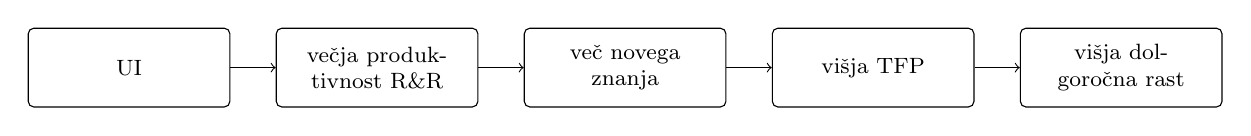
\begin{tikzpicture}[every node/.style={draw, rounded corners=2pt, align=center, font=\footnotesize, text width=2.35cm, minimum height=1cm, inner sep=3pt}]
\node (a) at (0,0) {UI};
\node (b) at (3.15,0) {večja produktivnost R\&R};
\node (c) at (6.3,0) {več novega znanja};
\node (d) at (9.45,0) {višja TFP};
\node (e) at (12.6,0) {višja dolgoročna rast};
\foreach \i/\j in {a/b,b/c,c/d,d/e} \draw[->] (\i) -- (\j);
\end{tikzpicture}
\caption{Vzročna veriga, ki jo preizkušamo}\label{fig:veriga}
\end{figure}

\begin{table}[H]
\centering
\caption{Hipoteze o vlogi UI in njihove napovedi}\label{tab:hipoteze}
\small
\renewcommand{\arraystretch}{1.2}
\begin{tabularx}{\textwidth}{>{\raggedright\arraybackslash}p{3.1cm} >{\raggedright\arraybackslash}X >{\raggedright\arraybackslash}X}
\toprule
Hipoteza & Mehanizem v modelu & Napoved za podatke \\
\midrule
\textbf{H1:} UI ne spremeni dolgoročne rasti & $x$ ostane nespremenjen, oziroma $\varphi+\beta<1$; več inputov dvigne raven, ne pa rasti & Rast TFP se med podobdobji sistematično ne spremeni, kljub rasti R\&R in UI-patentov \\
\textbf{H2:} UI poveča stopnjo tehnološkega napredka $x$ & Enkraten dvig $x$ za $\Delta x$ (enačbi~\eqref{eq:gY} in~\eqref{eq:racrasti}) & Stopničast dvig rasti TFP za $(1-\alpha)\Delta x$, brez nadaljnjega pospeševanja \\
\textbf{H3:} UI poveča raziskovalne inpute ali njihovo produktivnost & $\gamma$ je sorazmerna z $s\,l^{1-\varphi}$ (enačba~\eqref{eq:gamma}) & Rast R\&R in UI-patentov sledi (z zamikom) višja rast TFP, sorazmerna dvigu inputa \\
\textbf{H4:} UI poveča donose znanja ($\varphi+\beta>1$) & $\gamma$ narašča z akumulacijo znanja $h$ & Rast TFP narašča skozi čas: 2010--2014 $<$ 2015--2019 $<$ 2020--2025 \\
\bottomrule
\end{tabularx}
\caption*{\footnotesize Vir: lastna zasnova na podlagi \parencites{polanec_rast}{garin2021}.}
\end{table}

Pri H2--H4 se učinek lahko pokaže z zamikom, ker splošnonamenske tehnologije zahtevajo komplementarne investicije \parencite[str.~28]{polanec_rast}. Odsotnost učinka v kratkem obdobju zato hipotez ne ovrže, vztrajna odsotnost v daljšem obdobju pa jih oslabi. Patenti so le merljiv in delen izid raziskovanja, saj v Romerjevem modelu predstavljajo zaščito inovacije \parencite[str.~27--28]{polanec_rast}. Ker TFP vsebuje tudi druge dejavnike (razdelek~\ref{sec:viri}), preizkus pokaže le skladnost podatkov s posamezno hipotezo, ne vzročnosti.
\section{Uporaba modela in povezava s podatki}\label{sec:uporaba}

\subsection{R\&R in ustvarjanje novega znanja}

Empirične ugotovitve lahko najprej povežemo z osnovnim mehanizmom endogene teorije rasti. V Romerjevem okviru podjetja vlagajo v R\&R, ker pričakujejo prihodnje donose iz novih proizvodov, postopkov in drugih oblik novega znanja. Močna rast širših ameriških izdatkov za R\&R zato pomeni povečanje virov, ki so na voljo za raziskovalni proces.

Naslednji korak je pretvorba raziskovalnih inputov v novo znanje. Rast UI-patentne aktivnosti je skladna s tem, da se je povečala količina formaliziranih tehnoloških rezultatov, povezanih z umetno inteligenco. Patenti imajo v teoriji dvojno vlogo: inovatorju začasno omogočajo donos, hkrati pa z razkritjem znanja prispevajo k širjenju informacij in prihodnjim raziskavam. Zaradi takšnih prelivanj je lahko družbeni učinek raziskovanja večji od zasebnega učinka posameznega podjetja.

\subsection{Umetna inteligenca in produktivnost raziskovalnega procesa}

Za našo raziskovalno temo je ključno, da umetne inteligence ne obravnavamo le kot končni proizvod ali novo tehnologijo v proizvodnji, temveč tudi kot input v sam proces R\&R. Če UI omogoči hitrejšo obdelavo podatkov in literature, avtomatizacijo rutinskih nalog, simuliranje rešitev ali učinkovitejše programiranje, lahko raziskovalci z enako količino dela in kapitala ustvarijo več novega znanja.

V jeziku endogene teorije rasti to pomeni večjo produktivnost raziskovalnega sektorja. Rast federalnega financiranja UI R\&R in širjenje UI-patentne aktivnosti sta zato skladna z možnostjo, da se je povečal tako obseg raziskovalnih inputov kot tudi potencial za učinkovitejše ustvarjanje idej. Iz agregatnih podatkov pa ne moremo ločeno izmeriti, kolikšen del rasti novega znanja izhaja prav iz večje produktivnosti raziskovanja in kolikšen iz večjega obsega vloženih sredstev.

\subsection{Prenos novega znanja v TFP}

Tretji korak je prenos novega znanja v produktivnost proizvodnega sektorja. Če UI izboljša tehnologijo proizvodnje ali poveča učinkovitost raziskovanja, bi se njen dolgoročni učinek moral odraziti v TFP. Toda podatki ne kažejo preprostega sočasnega premika: raziskovalni in inovacijski kazalniki so v analiziranem obdobju močno rasli, rast TFP pa je bila precej bolj neenakomerna.

Takšen rezultat je skladen z idejo splošnonamenske tehnologije iz profesorjevih zapiskov. Širše tehnološke spremembe pogosto zahtevajo komplementarne investicije, reorganizacijo in učenje, zato se lahko njihovi produktivnostni učinki pojavijo šele z zamikom \parencite{polanec_rast}. Pri UI to vključuje podatkovno infrastrukturo, računsko moč, programsko opremo, spremembe delovnih procesov in usposabljanje zaposlenih.

\subsection{Primerjava napovedi modela z ugotovitvami}

Podatki so najbolj skladni s prvima členoma teoretičnega mehanizma. Viri za R\&R so se povečali, federalno financiranje raziskav UI je doseglo večmilijardne zneske, merljiva UI-povezana patentna aktivnost pa se je močno razširila. Manj jasen je zadnji člen, torej prenos teh sprememb v trajno višjo agregatno TFP.

\begin{table}[H]
\centering
\caption{Primerjava napovedi modela z empiričnimi ugotovitvami}
\small

\begin{tabular}{
>{\raggedright\arraybackslash}p{3.0cm}
>{\raggedright\arraybackslash}p{4.3cm}
>{\raggedright\arraybackslash}p{5.1cm}
}
\hline

\textbf{Člen mehanizma} &
\textbf{Napoved modela} &
\textbf{Opaženo v ZDA} \\

\hline

Raziskovalni inputi &
Več vlaganj v R\&R poveča vire za ustvarjanje novega znanja. &
Skupni izdatki za R\&R so se povečali s približno 406,6 mrd USD leta 2010 na 937 mrd USD leta 2023. \\

\hline

UI-specifični R\&R &
Več vlaganj v UI poveča raziskovalne zmogljivosti in potencial za inoviranje. &
Federalna vlaganja v UI R\&R so po letu 2019 dosegla večmilijardne ravni. \\

\hline

Ustvarjanje novega znanja &
Več oziroma učinkovitejši R\&R vodi v več inovacij. &
UI-povezana patentna aktivnost se je močno povečala; leta 2023 je bilo prepoznanih več kot 210.000 patentnih dokumentov. \\

\hline

Produktivnost &
Novo znanje se lahko dolgoročno odrazi v višji TFP. &
Povprečna rast TFP je bila 0,80 \% v obdobju 2010--2014, 0,64 \% v obdobju 2015--2019 in 1,00 \% v obdobju 2020--2025. Povezava je zato manj jasna. \\

\hline
\end{tabular}

\label{tab:model_podatki}
\end{table}

Tabela pokaže, da se empirični podatki najbolje ujemajo s prvima členoma teoretičnega mehanizma. Rast raziskovalnih inputov in UI-povezane inovacijske aktivnosti je izrazita, medtem ko je prenos v višjo agregatno TFP manj neposreden. To je skladno z možnostjo časovnega zamika med nastankom novega znanja in njegovim širšim učinkom na produktivnost. \\

Naše ugotovitve zato ne potrjujejo močne trditve, da je UI v obdobju 2010--2025 že povzročila trajen skok ameriške TFP. So pa skladne s šibkejšo in ekonomsko bolj utemeljeno trditvijo: povečali so se raziskovalni inputi in merljivo ustvarjanje UI-povezanega znanja, učinek na agregatno produktivnost pa je zaradi implementacijskih zamikov, merilnih težav in drugih makroekonomskih šokov težje izolirati. Takšno zaporedje dopuščata tako endogena teorija rasti kot koncept splošnonamenske tehnologije.

\section{Kritična presoja in zaključek}\label{sec:zakljucek}

\subsection{Odgovor na raziskovalno vprašanje}

Raziskovalno vprašanje je bilo, ali rast vlaganj v umetno inteligenco in širjenje inovacij, povezanih z UI, v ZDA v obdobju 2010--2025 spremljata povečano ustvarjanje novega znanja in rast skupne faktorske produktivnosti ter kako lahko to povezavo pojasnimo z modelom endogene gospodarske rasti.

Analiza pokaže, da je prvi del povezave v podatkih precej jasen. Ameriški izdatki za R\&R so se močno povečali, federalna vlaganja v UI R\&R pa so po letu 2019 dosegla večmilijardne ravni. Hkrati je močno narasla tudi UI-povezana patentna aktivnost, kar je skladno z večjim ustvarjanjem formaliziranega tehnološkega znanja.

Pri TFP je odgovor bolj zadržan. V novejšem obdobju je mogoče opaziti nekoliko višjo povprečno rast, vendar je serija zelo volatilna in močno zaznamovana s pandemskimi šoki. Podatki zato ne kažejo jasnega in takojšnjega prenosa rasti UI in R\&R v trajno višjo agregatno TFP. Ugotovitve so vseeno skladne z endogenim mehanizmom, po katerem večji raziskovalni inputi in učinkovitejše ustvarjanje znanja lahko dolgoročno povečajo produktivnost, pri čemer se učinek lahko pokaže z zamikom.

\subsection{Presoja in omejitev analize}
Endogena teorija rasti dobro pojasni predvsem povezavo med vlaganji v R\&R, ustvarjanjem novega znanja in dolgoročnim tehnološkim napredkom. Za naš primer je posebej uporabna razlaga umetne inteligence kot inputa v raziskovalni proces, saj lahko UI poveča produktivnost raziskovanja in s tem potencialno pospeši nastajanje novega znanja. Koncept splošnonamenske tehnologije hkrati pojasni, zakaj se povečanje vlaganj in inovacijske aktivnosti ne odrazi nujno takoj v višji agregatni TFP, ampak se lahko učinek pokaže šele z zamikom.

\begin{itemize}
    \item Največja omejitev analize je, da gre za opisno primerjavo časovnih vrst. Sočasna rast UI-kazalnikov, patentov in TFP ne pomeni, da je umetna inteligenca povzročila rast produktivnosti. Vzročnost je lahko dvosmerna: višja produktivnost in dobički lahko podjetjem omogočijo več investicij v R\&R, več vlaganj pa lahko pozneje spodbudi nadaljnjo produktivnost. Poleg tega na TFP vplivajo številni drugi dejavniki, zato brez kontrolne skupine, mikroekonomskih podatkov ali ustrezne identifikacijske strategije vzročnega učinka ne moremo oceniti.

    \item Druga omejitev je merjenje umetne inteligence. Federalni proračunski izdatki, patentni dokumenti in dejanska uporaba UI v podjetjih merijo različne faze inovacijskega procesa. Rast enega kazalnika zato ne pomeni nujno enake rasti vseh drugih. Posebej pazljivi moramo biti pri FY2025, kjer NITRD objavlja proračunsko zahtevo in ne realizirane porabe.

    \item Tretja omejitev je časovni zamik. Profesorjevi zapiski pri splošnonamenskih tehnologijah poudarjajo stroške razvoja komplementarnih inputov, namestitve in učenja \parencite{polanec_rast}. Pri UI lahko to pomeni investicije v podatkovno infrastrukturo, računsko moč, programsko opremo, organizacijske spremembe in usposabljanje zaposlenih. Posledično lahko patentna in investicijska aktivnost naraščata več let pred tem, ko se učinek v večjem obsegu pokaže v agregatni TFP.

    \item Četrta omejitev je sama narava TFP. Ker gre za rezidual, se vanjo prenesejo napake pri merjenju kapitala, dela in kakovosti inputov. TFP poleg tehnologije zajema tudi organizacijo, alokacijo virov, ekonomije obsega in druge spremembe učinkovitosti. Zato ni pravilno vsakega povečanja TFP neposredno interpretirati kot tehnološki napredek, še manj pa kot učinek UI.

    \item Peta omejitev so patenti. Patentni dokumenti ne zajamejo vseh inovacij, saj podjetja del znanja varujejo drugače, nekatera znanja pa sploh niso patentabilna. Tudi med patentiranimi izumi so velike razlike v gospodarski vrednosti. Število patentov je zato predvsem količinski indikator in ne neposredna mera kakovosti oziroma ekonomskega pomena novega znanja.
\end{itemize}
Nazadnje je pomembna dolžina analiziranega obdobja. Največji razmah generativne UI se je zgodil šele v zadnjih letih, zato je leto 2025 verjetno prezgodnje za zanesljivo presojo dolgoročnega makroekonomskega učinka. Močni učinki se lahko najprej pokažejo v posameznih panogah in podjetjih, v agregatni TFP pa šele pozneje.

\subsection{Zaključek}

Rezultati kažejo, da je ameriško gospodarstvo v obdobju 2010--2025 povečalo tako širše vire za R\&R kot dejavnosti, neposredno povezane z umetno inteligenco. Hkrati se je razširila merljiva UI-povezana inovacijska aktivnost. To je skladno z napovedjo endogene teorije rasti, da vlaganja v raziskovanje in ustvarjanje znanja predstavljajo pomemben vir tehnološkega napredka.

Najbolj previdni moramo biti pri sklepanju o agregatni produktivnosti. Trenutni podatki še ne omogočajo trditve, da je umetna inteligenca povzročila trajen skok TFP. Bolj utemeljen sklep je, da se je okrepil raziskovalni in inovacijski del mehanizma, medtem ko je morebitni dolgoročni produktivnostni učinek še težko ločiti od časovnih zamikov in drugih gospodarskih sprememb. Nadaljnje raziskave bi bilo zato smiselno usmeriti v sektorske in podjetniške podatke ter makroekonomsko primerjavo ponoviti čez nekaj let.

\newpage
\printbibliography[title={Literatura in viri}, heading=bibintoc]

\end{document}